\documentclass{jvfscript-de}
%=======================================================================================================%
%                                                                                                       %
% Dieses Skript benötigt mein Package jvftex, erhältlich unter https://github.com/vonfalkenstein/jvftex %
%                                                                                                       %
%=======================================================================================================%
\usepackage{ztstyle}
\usepackage{graphicx}
\graphicspath{ {./images/} }

%\usepackage{showframe}

\makeindex[title=Definitionen,intoc]
\DeclareNewTOC[owner=jvfscript-de,listname=Dateiverzeichnis,type=files,types=files, name=Datei]{listoffiles}
\newcounter{file}
\newcounter{video}
\newcommand{\file}[1]{%
	\stepcounter{file}
	\marginnote{\normalfont Datei \thefile: #1}
	\addxcontentsline{listoffiles}{section}[]{Datei \thefile{} - {#1}}
}
\newcommand{\video}{%
	\stepcounter{video}
	\marginnote{\normalfont Video \thelecture\_\thevideo}
}
\newcommand{\filevideo}[1]{%
	\stepcounter{file}
	\stepcounter{video}
	\marginnote{\normalfont Datei \thefile: #1,\\Video \thelecture\_\thevideo}
	\addxcontentsline{listoffiles}{section}[]{Datei \thefile{} - {#1}}
}
\newcommand{\lecturefile}[2]{%
	\stepcounter{file}
	\stepcounter{lecture}
	\marginnote{\normalfont Vorlesung \thelecture, #1, Datei \thefile: #2}
	\addxcontentsline{listoflectures}{section}[]{Vorlesung \thelecture{} vom #1}
	\addxcontentsline{listoffiles}{section}[]{Datei \thefile{} - {#2}}
}
\newcommand{\lecturevideo}[1]{%
	\setcounter{video}{0}
	\stepcounter{lecture}
	\stepcounter{video}
	\marginnote{\normalfont Vorlesung \thelecture, #1, Video \thelecture\_\thevideo}
	\addxcontentsline{listoflectures}{section}[]{Vorlesung \thelecture{} vom #1}
}
\newcommand{\lecturefilevideo}[2]{%
\setcounter{video}{0}
\stepcounter{file}
\stepcounter{lecture}
\stepcounter{video}
\marginnote{\normalfont Vorlesung \thelecture, #1, Datei \thefile: #2, Video \thelecture\_\thevideo}
\addxcontentsline{listoflectures}{section}[]{Vorlesung \thelecture{} vom #1}
\addxcontentsline{listoffiles}{section}[]{Datei \thefile{} - {#2}}
}

%\renewcommand{\thechapter}{\S \arabic{chapter}}
%\renewcommand{\thesection}{\arabic{chapter}.\arabic{section}}
\renewcommand{\thethm}{\arabic{chapter}.\arabic{thm}}

\hypersetup{
	pdftitle={Vorlesungsskript Zahlentheorie}
}



%\includeonly{./lectures/cpt04}

\usetikzlibrary{patterns}
%\usepackage[dvipsnames]{xcolor}
\usepackage{pgfplots}

\begin{document}
\frontmatter
	\maketitle
	\begingroup
	\let\clearpage\relax
	\tableofcontents
	\listoflectures
	\listoffiles
	\endgroup
\newpage
\thispagestyle{plain}

Dieses Skript stellt keinen Ersatz für die Vorlesungsnotizen von Prof. Schindler dar und wird nicht nochmals von ihr durchgesehen. Im Grunde sind das hier nur meine persönlichen Mitschriften, ich garantiere also weder für Korrektheit noch Vollständigkeit und werde ggf. noch weitere Beispiele und Anmerkungen einfügen. Beweise werde ich in der Regel nicht übernehmen (weil das in \LaTeX{} einfach keinen Spaß macht).

Falls Ihr Korrekturanmerkungen habt könnt Ihr mir gern bei \href{https://studip-ecampus.uni-goettingen.de/dispatch.php/profile?username=n.sennewald}{Stud.IP} schreiben oder direkt im \href{https://github.com/vonfalkenstein/Vorlesungsmitschrift-Zahlentheorie}{GitHub Repository} einen pull request machen (was für mich deutlich weniger umständlich ist als der Weg über Stud.IP).\\\\
glhf,\\
Alex

\vspace{\fill}
\begin{quote}
	"Die Zahlentheorie ist nützlich, weil man mit ihr promovieren kann."
\end{quote}\hspace{\fill} --Edmund Landau
\vspace{\fill}


\mainmatter
	
	\chapter{Primzahlen - Bausteine der ganzen Zahlen}\lecturefilevideo{13.04.2021}{Primzahlen \& Teilbarkeit}

%\[ \begin{tikzcd}
%	&&&G/\ker f \arrow{ddr}{\iota}&\\
%	\\
%	\ker f \arrow{rr}{\kappa}&& G \arrow{rr}{f} \arrow{uur}{\pi}& & H
%\end{tikzcd} \]

Wo ergeben sich für uns in der Zahlentheorie Unterschiede, wenn wir über $\Z$ anstatt über $\Q$ arbeiten?

\begin{exmp*}
	Seien $a,b \in \Z$, $a\neq 0$. Dann hat die Gleichung
	\[ ax = b \]
	nicht immer eine Lösung $x \in \Z$.
\end{exmp*}

\begin{defn*}[Teiler]\index{Teiler}
	Seien $a,b \in \Z$. Wir sagen, dass \emph{$\emph{a}$ ein Teiler von $\emph{b}$ ist} ($a \mid b$), falls es eine ganze Zahl $x \in \Z$ gibt mit $ax = b$.
\end{defn*}

\begin{lem}\autolabel
	Seien $a,b,c,d \in \Z$.
	\begin{enumerate}[label={\roman*})]
		\item Falls $d \mid a$ und $d \mid b$, dann $d \mid a+b$.
		\item Ist $d \mid a$, dann auch $d \mid ab$.
		\item Ist $d \mid a$, dann gilt $db \mid ab$.
		\item Gilt $d \mid a$ und $a \mid b$, dann $d \mid b$.
		\item Ist $a \neq 0$ und $d \mid a$, dann gilt $|d| \leq |a|$.
	\end{enumerate}
\end{lem}

\begin{rem*}
	Eine ganze Zahl $a \neq 0$ hat höchstens endlich viele Teiler.
\end{rem*}

\begin{thm}[Teilen mit Rest]\autolabel
	Seien $a,b \in \Z, b > 0$. Dann gibt es $q,r \in \Z$ mit
	\[ a = bq + r, \ 0 \leq r < b. \]
\end{thm}

\begin{defn*}[Primzahl]\index{Primzahl}\video
	Eine ganze Zahl $p > 1$, die genau zwei positive Teiler hat (1 und sich selbst), nenn wir \emph{Primzahl}.
\end{defn*}

\begin{exmp*}
	\( 2,3,5,7,11,13,17,19,23,29,31,\dotsc \)
\end{exmp*}

\begin{lem}\autolabel
	Sei $n \in \N, n > 1$ und sei $p>1$ der kleinste positive Teiler von $n$. Dann ist $p$ eine Primzahl. Ist außerdem $n$ nicht prim, dann gilt $p \leq \sqrt{n}$.
\end{lem}

\begin{rem*}
	Diese Eigenschaft findet Anwendung im \emph{Sieb von Eratosthenes}. Dies ist ein einfacher Algorithmus, um schnell alle Primzahlen bis $n$ zu finden. Hierfür definieren wir zunächst die Menge \( A = \{z \in \Z \mid 2 \leq z \leq n\} \). Durch Lemma \ref{1.3} genügt es, zusätzlich lediglich die Menge $B = \{k \cdot p \mid k \in \Z, p \leq \sqrt{n} \ \text{prim}\}$, also alle Primzahlen $p \leq \sqrt{n}$ und deren Vielfache zu betrachten. Die Differenz $A \setminus B$ beinhaltet dann nur noch alle Primzahlen $\sqrt{n} \leq p \leq n$.
\end{rem*}

\begin{thm}[Euklid]\autolabel
	Es gibt unendlich viele Primzahlen.
\end{thm}

\begin{thm}[Hauptsatz der Arithmetik, Primfaktorzerlegung]\autolabel
	Jede natürliche Zahl $n > 1$ kann auf eindeutige Weise als Produkt
	\[ n = p_1^{k_1} \cdot p_2^{k_2} \dotsm p_r^{k_r} \]
	mit $k_1, \dotsc, k_r \in \N$ und $p_1 < p_2 < \dots < p_r$ Primzahlen geschrieben werden.
\end{thm}

\begin{lem}\video\autolabel
	Seien \( a,b, p \in \N \) und $p$ eine Primzahl. Angenommen $p \mid ab$, dann gilt $p \mid a$ oder $p \mid b$.
\end{lem}

\begin{cor}\autolabel
	Seien $a_1,\dotsc,a_n \in \N$ und $p$ eine Primzahl mit $p \mid a_1 \dotsm a_n$. Dann $\existss 1 \leq i \leq n$ mit $p \mid a_i$.
\end{cor}

\begin{thm}\autolabel
	Seien $a, b \in \N$ mit Primfaktorzerlegungen
	\[ a = p_1^{a_1} \cdot p_2^{a_2} \dotsm p_r^{a_r},\quad b = p_1^{b_1} \cdot p_2^{b_2} \dotsm p_r^{b_r} \]
	mit $p_1, \dotsc,r_p$ Primzahlen, $p_i \neq p_j$ für $i \neq j$ und $a_i,b_i \geq 0\ \foralll i$. Dann gilt genau dann \( b \mid a \), wenn \( b_i \leq a_i \ \foralll i \).
\end{thm}

\subsection*{Der größte gemeinsame Teiler}\video

\begin{defn*}[größter gemeinsamer Teiler]\index{größter gemeinsamer Teiler}
	Seien $a,b \in \N$. Der \emph{größte gemeinsame Teiler von $\emph{a}$ und $\emph{b}$} ist der größte Teiler $d$ mit $d \mid a$ und $d \mid b$. Wir schreiben $\ggt(a,b) = d$ (im englischen $\gcd(a,b)$).
\end{defn*}

\begin{rem*}
Seien $a = p_1^{a_1} \cdot p_2^{a_2} \dotsm p_r^{a_r},\quad b = p_1^{b_1} \cdot p_2^{b_2} \dotsm p_r^{b_r}$ mit $p_1, \dotsc,r_p$ Primzahlen, $p_i \neq p_j$ für $i \neq j$ und $a_i,b_i \geq 0\ \foralll 1 \leq i \leq r$, und $d \in \N$ mit $ d = p_1^{d_1} \cdot p_2^{d_2} \dotsm p_r^{d_r}$, wobei $d_i \geq 0 \ \foralll 1 \leq i \leq r$. Angenommen $d \mid a$ und $d \mid b$, dann $d_i \leq a_i,b_i \ \foralll 1 \leq i \leq r$. Ist $d = \ggt(a,b)$, dann gilt $d_i = \min(a_i,b_i) \ \foralll 1 \leq i \leq r$ und 
$$\ggt(a,b) = p_1^{\min(a_1,b_1)} \cdot p_2^{\mid(a_2,b_2)} \dotsm p_r^{\min(a_r,b_r)}.$$
\end{rem*}

\begin{lem}\autolabel
	Seien $a,b,c,d \in \N$.
	\begin{enumerate}[label={\roman*})]
		\item Ist $d \mid a$ und $d \mid b$, dann $d \mid \ggt(a,b)$.
		\item Angenommen $b \mid ac$ und $\ggt(a,b) = 1$. Dann gilt $b \mid c$.
		\item Sei $a \mid c,\ b \mid c$ und $\ggt(a,b) = 1$. Dann $ab \mid c$.
		\item Sei $d = \ggt(a,b)$. Dann gilt \( \ggt \left( \frac{a}{d},\frac{b}{d} \right) = 1. \)
	\end{enumerate}
\end{lem}

\subsection*{Das kleinste gemeinsame Vielfache}

\begin{defn*}[kleinstes gemeinsames Vielfaches]\index{kleinstes gemeinsames Vielfaches}
	Seien $a,b \in \N$. Die kleinste natürliche Zahl $m$ mit $a \mid m$ und $b \mid m$ nennen wir das \emph{kleinste gemeinsame Vielfache von $\emph{a}$ und $\emph{b}$}. Wir schreiben $\kgv(a,b) = m$ (im englischen $\lcm(a,b)$).
\end{defn*}

\begin{rem*}
	Seien $a,b$ mit den gleichen Primfaktorzerlegungen wie oben. Dann
	\[ \kgv(a,b) = p_1^{\max(a_1,b_1)} \cdot p_2^{\max(a_2,b_2)} \dotsm p_r^{\max(a_r,b_r)}. \]
	Bemerke: $\max(a_i,b_i) + \min(a_i,b_i) = a_i + b_i$. Also $ab = \ggt(a,b) \cdot \kgv(a,b)$.
\end{rem*}

\begin{defn*}
	Seien \( a_1,\dotsc,a_k \in \Z \), nicht alle gleich null. Der größte gemeinsame Teiler von \( a_1,\dotsc,a_k \) ist die größte natürliche Zahl $d$, die jedes der $a_i$ teilt. Wir schreiben \( d = \ggt(a_1,\dotsc,a_k) \). Analog dazu können wir das kleinste gemeinsame Vielfache von $a_1,\dotsc, a_k$ als die kleinste positive ganze Zahl $m$ definieren, die durch jedes der $a_i$ teilbar ist, $m = \kgv(a_1,\dotsc,a_k)$.
\end{defn*}

\section*{Der Euklidische Algorithmus}\filevideo{Der Euklidische Algorithmus}

\emph{Motivation:} Seien $a,b \in \N$. Wie können wir $\ggt(a,b)$ schnell berechnen?

\begin{rem*}
	Für $a,b \in \N$ schreibe $a = qb + r$ mit $0 \leq r < b$.
	\begin{enumerate}[label={\roman*})]
		\item Ist $d \in \N$ mit $d \mit a$ und $d \mid b$, dann gilt auch $d \mid r$.
		\item Ist $d \mid b$ und $d \mid r$, dann $d \mid a$.
	\end{enumerate}
	Es folgt: $\ggt(a,b) = \ggt(b,r)$.
\end{rem*}

\begin{exmp*}
	$a = 270,\ b = 192$
	\begin{align*}
		270 &= 1 \cdot 192 + 78\\
		192 &= 2 \cdot 78 + 36\\
		78 &= 2 \cdot 36 + 6\\
		36 &= 6 \cdot 6 + 0\\
		\noalign{\centering $\implies \ggt(270,192) = \dotsc = \ggt(6,0) = 6$}
	\end{align*}
\end{exmp*}

Im Allgemeinen sieht das wie folgt aus:
\begin{align*}
	a &= q_0 b + r_1\\
	b &= q_1 r_1 + r_2\\
	r_1 &= q_2 r_2 + r_3\\
	\noalign{\centering \dots}
	r_{k-2} &= q_{k-1} r_{k-1} + r_k\\
	r_{k-1} &= q_k r_k + 0\\
	\implies \ggt(a,b) &= r_k
\end{align*}
Warum endet der Euklidische Algorithmus nach endlich vielen Schritten? In jedem Schritt gilt $0 \leq r_{j+1} < r_j \ \foralll j$. Da wir mit einer endlichen Zahl $b$ angefangen haben ist auch unser $r_1$ endlich, und da sich der Rest in jedem Schritt um mindestens 1 verkleinert sind wir nach maximal $|b|$ Schritten fertig.

Der Euklidische Algorithmus ist schnell. Sei $a > b$, dann ist $r_1 < \frac{a}{2}$. Wenn wir dies fortsetzen erhalten wir 
\begin{align*}
	r_2 &< r_1 < \frac{a}{2}\\
	r_3 &< \frac{r_1}{2} < \frac{a}{4}\\
	r_4 &< \frac{r_2}{2} < \frac{a}{4}\\
	\dots
\end{align*}
Nach Vollständiger Induktion folgt 
\[ r_m < \frac{a}{2^{\frac{m}{2}}}\qquad \foralll m>0. \]
Daher \( 1 \leq r_k < \frac{a}{2^{\frac{k}{2}}} \), also \( 2^\frac{k}{2} < a \) und somit
\[ k < 2\frac{\log a}{\log 2} \]
	\chapter{Die Teilerfunktion} \filevideo{Teilerfunktion, Kongruenzen}

\begin{defn*}[Teilerfunktion]\index{Teilerfunktion}
	Sei $n \in \N$. Wir definieren \( d(n) \) als die Zahl der positiven Teiler von $n$, d.h.
	\[ d(n) = \sum_{\substack{d \mid n \\ d \geq 1}} 1. \]
	Weiter definieren wir
	\[ S(n) = \sum_{\substack{d \mid n \\ d \geq 1 \\ d < n}} d \]
	und 
	\[ \sigma(n) = \sum_{\substack{d \mid n \\ d \geq 1}} d \]
\end{defn*}

\begin{exmp*}
	\( d(7) = 2,\ d(6) = 4 \)\\
	Sei $p$ eine Primzahl, dann gilt $d(p) = 2$ und $d(p^k) = k+1$ für $k\geq 0$.
\end{exmp*}

\begin{rem*}
	$\sigma(n) = S(n) + n$
\end{rem*}

\begin{defn*}[perfekte Zahl] \index{perfekte Zahl}
	Wir nennen eine natürliche Zahl $n$ \emph{perfekt}, falls
	\[ S(n) = n. \]
\end{defn*}

\begin{exmp*}
	$6 = 1+2+3$ ist perfekt. 28 ist perfekt.
\end{exmp*}

\begin{lem}\autolabel
	Seien $m,n \in \N$ mit $\ggt(m,n) = 1$. Dann gilt
	\[ d(mn) = d(m)d(n) \]
	und \[ \sigma(mn) = \sigma(m) \sigma(n). \]
\end{lem}

\begin{rem*}
	$d(n)$ und $\sigma(n)$ sind sogenannte \textit{multiplikative Funktionen}.
\end{rem*}

Kennt man die Primfaktorzerlegung von $n$, so lassen sich diese Funktionen sehr einfach berechnen. Wir wollen nun eine allgemeine Formel für $d(n)$ aufstellen.

Sei $n = p_1^{k_1} \dotsm p_r^{k_r}$ mit $p_1 < \dots < p_3$ Primzahlen, $k_1, \dotsm, k_r \geq 0$. Dann gilt nach Lemma \ref{2.1}
\begin{align*}
	d(n) &= d \left( p_1^{k_1} \dotsm p_r^{k_r} \right)\\
	&= d\left(p_1^{k_1}\right) \dotsm d\left(p_r^{k_r}\right)
\end{align*}
Es gilt
\[ d(p^k) = k + 1, \]
also
\[ d(n) = (k_1+1) (k_2+1) \dotsm (k_r+1). \]
Weiterhin berechnen wir
\begin{align*}
	\sigma(n) &= \sigma\left(p_1^{k_1}\right) \dotsm \sigma\left(p_r^{k_r}\right)\\
	\sigma\left(p^k\right) &= 1 +p + p^2 + \dots + p^k\\
	&= \frac{p^{k+1} -1}{p-1}
\end{align*}
Wir erhalten
\[ \sigma(n) = \frac{p_1^{k_1+1} - 1}{p_1-1} \dotsm \frac{p_r^{k_r+1}-1}{p_r-1} \]

\begin{thm}\autolabel
	Sei $n = p_1^{k_1} \dotsm p_r^{k_r}$ mit $p_1 < \dots < p_3$ Primzahlen, $k_1, \dotsm, k_r \geq 0$. Dann gilt 
	\begin{align*}
		d(n) &= \prod_{i=1}^r (k_i+1)\\
		\sigma(n) &= \prod_{i=1}^r \frac{p_i^{k_i + 1}-1}{p_i-1}.
	\end{align*}
\end{thm}

\begin{exmp*}
	\( d(25 \cdot 3) = d(25) d(3) = d(5^2) d(3) = 3 \cdot 2 = 6 \)
\end{exmp*}

\begin{rem*}
	$S(n)$ ist keine multiplikative Funktion:\\
	\( 1 = S(2)S(3) \neq S(6) = 6 \)
\end{rem*}
	\chapter{Kongruenzen}\video

\begin{exmp*}
	Die Uhr
	\incfig{3_1}{10cm}
	Der Minutenzeiger weiß nur, wie viele Minuten es nach einer vollen Stunde ist
\end{exmp*}

\begin{defn*}[Kongruenz, Kongruenzklasse]\index{Kongruenzklasse}
	Sei $M \in \N,\ M > 1,\ a,b \in \Z$. Wir sagen, dass \emph{$\emph{a}$ kongruent zu $\emph{b}$ ist modulo $\emph{M}$}, falls \( M \mid (a-b) \), schreibe \( a \equiv b \bmod M \).\\
	Sei $r \in \Z$. Die Menge aller ganzen Zahlen $x$ mit $x \equiv r \bmod M$ nennen wir die \emph{Kongruenzklasse von $\emph{r}$ modulo $\emph{M}$}.
\end{defn*}

\begin{exmp*}
	\( 7 \equiv  27 \bmod 10,\ 4 \equiv 1 \bmod 3 \)
\end{exmp*}

\begin{lem}\autolabel
	Sei $M > 1,\ M \in \N,\ a_1,a_2,b_1,b_2 \in \Z$ mit $a_1 \equiv a_2 \bmod M$ und $b_1 \equiv b_2 \bmod M$. Dann gilt
	\begin{enumerate}[label={\roman*})]
		\item $a_1 + b_1 \equiv a_2 + b_2 \bmod M$
		\item $a_1 - b_1 \equiv a_2 - b_2 \bmod M$
		\item $a_1b_1 \equiv a_2b_2 \bmod M$
	\end{enumerate}
\end{lem}

\begin{notat*}
	Schreibe \( \Z / M\Z \) für die Menge aller Restklassen modulo $M$.
\end{notat*}

\emph{Eine Anwendung:} Eine natürliche Zahl $n$ ist durch 9 teilbar genau denn, wenn die Summe ihrer Ziffern in der Dezimaldarstellung (also ihre Quersumme) durch 9 teilbar ist.

\begin{exmp*}
	43227 ist durch 9 teilbar.
\end{exmp*}

\section{Inverse Restklassen}\filevideo{Inverse Restklassen}

Seien \( x,y \in \Z \) mit $2x = 2y $. Die echten Detektive unter uns erkennen, dass man dies einfach zu $x = y$ kürzen kann. Nun ist die Frage, ob das auch funktioniert, wenn wir statt über $\Z$ über dem Restklassenring arbeiten, also ob wir auch bei Kongruenzen kürzen können.

\begin{exmp*}
	\begin{enumerate}
		\item[]
		\item \( 2x \equiv 2y \bmod 4 \overset{?}{\implies} x \equiv y \bmod 4 \)\\
			\textcolor{red}{Nein $\lightning$}, z.B. \( 2 \cdot 3 \equiv 2 \cdot 1 \bmod 4,\ 3 \not\equiv 1 \bmod 4 \)
		\item \( 2x \equiv 2y \bmod 5 \implies 5 \mid 2(x-y) \), d.h. \( 5 \mid x-y \implies x \equiv y \bmod 5 \)\\
			\underline{oder} bemerke, dass \( 2 \cdot 3 \equiv 1 \bmod 5 \) und multipliziere die obige Kongruenz mit 3.
	\end{enumerate}
\end{exmp*}

\begin{defn*}[Invertierbare Restklasse]\index{Kongruenzklasse!Invertierbare Restklasse}
	Sei \( M \in \N,\ M > 1 \). Wir nennen \( a \in \Z \) \emph{invertierbar modulo $\emph{M}$}, falls es \( \existss b \in \Z \) gibt mit \( ab \equiv 1 \bmod M \). In dem Fall nennen wir die Restklasse \( a\) (modulo $M$) invertierbar.
\end{defn*}

\begin{exmp*}
	2 ist invertierbar modulo 25, denn \( 2 \cdot 13 \equiv 1 \bmod 25 \).
\end{exmp*}

\begin{thm}\autolabel
	Sei \( M \in \N,\ M > 1,\ a \in \Z \). Dann ist $a$ invertierbar modulo $M$ genau dann, wenn \( \ggt(a,M) = 1 \).
\end{thm}

\begin{rem*}
	Ist \( a \in \Z \) invertierbar modulo $M$, dann ist jedes Element in der Restklasse $a \bmod M$ invertierbar modulo $M$.\video Die Menge aller $b \in \Z$ mit $ba \equiv 1 \bmod M$ ist eine Restklasse modulo $M$, schreibe $a^{-1}$ (modulo $M$) für diese Restklasse.
\end{rem*}

Sei \( a \in \Z,\ M \in \N,\ M > 1 \) mit \( \ggt(a,M) = 1 \). Wie können wir die inverse Restklasse $a^{-1}$ berechnen?\\
$\implies$ wir verwenden den erweiterten Euklidischen Algorithmus um \( x,y \in \Z \) zu finden mit \( ax+My = 1 \).

\begin{notat*}
	Ist $M > 1$, so schreiben wir \( (\Z / M\Z)^* \) für die Menge der invertierbaren Restklassen modulo $M$.
\end{notat*}

\begin{exmp*}
	\begin{enumerate}
		\item[]
		\item \( (\Z/6\Z)^* = \left\{\bar{1},\bar{5}\right\} \), also \( |(\Z/6\Z)^*| = 2 \)
		\item Sei $p$ prim.
		\[ (\Z/p\Z)^* = \{1, 2, \dotsc, p-1 \} \implies |(\Z/p\Z)^*| = p-1 \]
	\end{enumerate}
\end{exmp*}

\begin{lem}[Satz von Wilson]\autolabel
	Sei $p$ prim. Dann gilt \( (p-1)! \equiv -1 \bmod p. \)
\end{lem}

\section{Lineare Kongruenzgleichungen}\lecturefilevideo{20.04.2021}{Lineare Kongruenzgleichungen}

\begin{frage*}
	Seien $a,b \in \Z,\ M \in \N$. Finde alle ganzzahligen Lösungen $x \in \Z$, sodass gilt
	\[ ax \equiv b \mod M. \]
\end{frage*}

\begin{exmp*}
	\begin{enumerate}[label={\roman*})]
		\item \( 5x \equiv 7 \bmod 15 \) hat \textit{keine} Lösung
		\item \( 5x \equiv 25 \bmod 15 \), d.h. \( 15 \mid (5x - 25) = 5(x-5) \iff 3 \mid x-5 \) oder \( x \equiv 5 \bmod 3 \), d.h. \( x \equiv 2 \bmod 3 \). Die Lösungen der Kongruenz \( 5x \equiv 25 \bmod 15 \) sind gegeben durch alle $x \in \Z$ der Form $x = 2+3k$ mit $k \in \Z$.
	\end{enumerate}
\end{exmp*}

\begin{thm}\autolabel
	Seien $a,b \in \Z,\ M \in \Z_{\geq 2}$ und $d = \ggt(a,M)$. Die Gleichung
	\[ ax \equiv b \mod M \]
	hat genau dann eine Lösung $x \in \Z$, wenn $d \mid b$.\\
	Wenn dies gilt, dann ist die Gleichung $ax \equiv b \bmod M$ äquivalent zu 
	\[ \frac{a}{d} x \equiv \frac{b}{d} \mod \frac{M}{d}. \]
	Diese Gleichung hat eine Lösung, denn
	\[ \ggt \left( \frac{a}{d}, \frac{M}{d} \right) = 1. \]
\end{thm}

\section{Der Chinesische Restsatz}\filevideo{Der Chinesische Restsatz}

Wir wollen alle $x \in \Z$ finden, die nach Teilen mit Rest durch 2,3,5 die Reste 1,2,3 lassen. Anders formuliert: Finde $x \in \Z$ mit
\begin{align*}
	x &\equiv 1 \mod 2\\
	x &\equiv 2 \mod 3\\
	x &\equiv 3 \mod 5
\end{align*}
Ist $x \in \Z$ eine Lösung der obigen Kongruenzen, dann auch $x + 30k$ für jedes $k \in \Z$.\\
Sei nun $x$ eine solche Lösung. Dann gilt $x \equiv 3 \bmod 5$, schreibe $x = 3+5u$ mit $u \in \Z$. Es muss außerdem gelten
\[ 3 + 5u \equiv 2 \mod 3, \]
d.h. $2u \equiv 2 \bmod 3 \iff u \equiv 1 \bmod 3,$ also $u = 1+3v$ mit $v \in \Z$, schreibe also
\begin{align*}
	x &= 3+5(1+3v)\\
	&= 8+15v.
\end{align*}
Zuletzt betrachten wir nun 
\[ 8+15v \equiv 1 \mod 2. \]
Daraus folgt, dass $v$ ungerade ist, d.h. $v = 1+2w$ mit $w \in \Z$. Wir erhalten
\begin{align*}
	x &= 8+15(1+2w)\\
	&= 23+30w,\quad w \in \Z.
\end{align*}

\subsection*{Im Allgemeinen:}

Seien $c_1,\dotsc,c_n \in \Z,\ m_1,\dotsc,m_n \in \Z_{\geq 2}$. Finde alle $x \in \Z$ mit
\begin{equation}\label{ChinRem}
	\begin{split}
		x &\equiv c_1 \mod m_1\\
		x &\equiv c_2 \mod m_2\\
%		\noalign{\centering $\vdots$}
		x &\equiv c_n \mod m_n
	\end{split}\tag{$*$}
\end{equation}
\emph{Achtung:} Es ist zu beachten, dass es manchmal keine Lösung gibt, z.B. bei 
\begin{align*}
	x &\equiv 1 \mod 3\\
	x &\equiv 2 \mod 9.
\end{align*}
Dies rührt daher, dass wir bisher keine Annahmen über die Module getroffen haben, was wir später noch für den chinesischen Restsatz tun werden. Zunächst fassen wir unsere Vorüberlegungen, dass sich unsere Lösungsmenge durchs kleinste gemeinsame Vielfache der Module ergibt, in folgendem Lemma zusammen:

\begin{lem}\autolabel
	Sei $x_0 \in \Z$ eine Lösung zum System \ref{ChinRem}. Dann besteht die gesamte Lösungsmenge des Systems aus der Restklasse $x_0 \bmod M$ mit $M = \kgv(m_1,\dotsc,m_n)$.
\end{lem}

\begin{thm}[Chinesischer Restsatz]\autolabel\video
	Wir benutzen die gleiche Notation wie im System \ref{ChinRem}. Angenommen, $\ggt(m_i,m_j)=1$ für $i \neq j$, dann hat das System \ref{ChinRem} genau eine Restklasse modulo $m_1 \dotsm m_n$ als Lösung.
\end{thm}
	\chapter{Die Eulersche $\varphi$-Funktion}\filevideo{Eulersche $\varphi$-Funktion}\footnote{Nach Leonhard Euler (1707-1783), ein Schweizer Mathematiker, Physiker, Astronom, Geograph, Logiker und Ingenieur}
\section*{Ordnungen und Primitivwurzeln}

\begin{frage*}
	Sei $M \geq 2$. Wie viele invertierbaren Restklassen gibt es modulo $M$?
\end{frage*}

\begin{notat*}
	Wir schreiben
	\[ \varphi(M) = |(\Z/M\Z)^*| = |\{0 < a \leq M \mid \ggt(a,M) = 1\}|. \]
\end{notat*}

\begin{exmp*}
	\begin{enumerate}[label={\roman*})]
		\item $\varphi(2) = 1, \varphi(3)=2, \varphi(4)=2, \varphi(5)=4, \varphi(6)=2$\\
		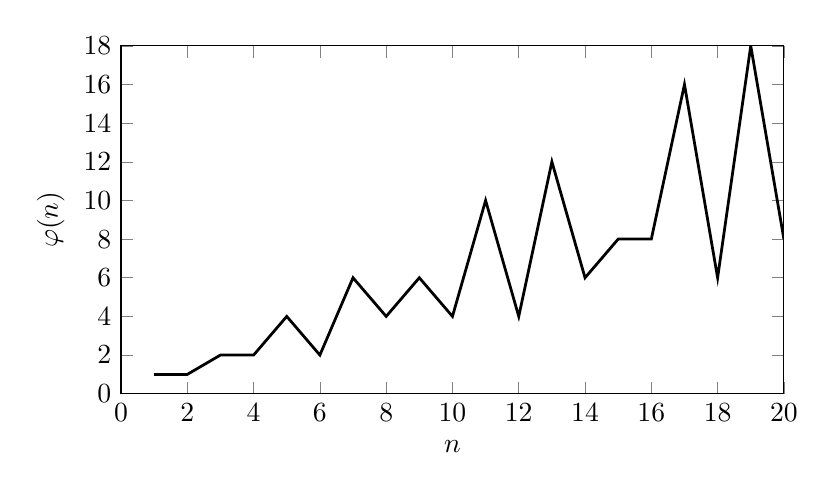
\begin{tikzpicture}
			\begin{axis}
				[
				xlabel={$n$}, ylabel={$\varphi(n)$}, xmin=0, xmax=20,
				ymin=0, ymax=18,
				height=6cm,
				width=10cm,
				xtick={0,2,4,6,8,10,12,14,16,18,20},
				ytick={0,2,4,6,8,10,12,14,16,18},
				]
				
				\addplot[line width=1pt]
				coordinates{
					(1,1) (2,1) (3,2) (4,2) (5,4) (6,2) (7,6) (8,4) (9,6) (10,4) (11,10) (12,4) (13,12) (14,6) (15,8) (16,8) (17,16) (18,6) (19,18) (20,8)};
			\end{axis}
		\end{tikzpicture}
		\item Sei $p$ eine Primzahl. Dann ist $\varphi(p) = p-1$.
		\item Sei $k \geq 1$ und $p$ prim. Dann gilt
			\begin{align*}
				\varphi(p^k) &= p^k - \left|\left\{0 < a \leq p^k \mid \ggt\left(a,p^k\right)>1\right\}\right|\\
				&= p^k - p^{k-1}
			\end{align*}
			Eine Beobachtung:
			\begin{align*}
				\varphi(1) + \varphi(p) + \varphi(p^2) + \dots + \varphi(p^k) &= 1 + (p-1) + (p^2-p) + \dots + (p^k-k^{k-1}) \\
				&= p^k
			\end{align*}
	\end{enumerate}
\end{exmp*}

\begin{thm}\autolabel
	Sei $n \in \Z$. Dann gilt
	\[ \sum_{d \mid n} \varphi(d) = n. \]
\end{thm}

Nun wollen wir uns mit der Berechnung der Eulerschen $\varphi$-Funktion beschäftigen. Für Primzahlpotenzen haben wir das schon getan und wollen dies jetzt auf allgemeine natürliche Zahlen anhand ihrer Primfaktorzerlegung fortsetzen.

\begin{thm}\autolabel\video
	$\varphi$ ist eine multiplikative Funktion, d.h. für $m,n \in \N$ mit $\ggt(m,n) = 1$ gilt $$\varphi(mn) = \varphi(m)\varphi(n).$$
\end{thm}

\begin{cor}
	Sei $m = p_1^{k_1} p_2^{k_2} \dotsm p_r^{k_r}$ mit $p_1 < p_1 < \dots < p_r$ Primzahlen und $k_i \geq 0$ für $1 \leq i \leq r$. Dann gilt
	\begin{align*}
		\varphi(m) &= \prod_{i=1}^r \left( p_i^{k_1} - p_i^{k_i-1} \right)\\
		\noalign{\centering oder}
		\varphi(m) &= m \cdot \prod_{\substack{p \mid  m \\ p \ \text{prim}}} \left( 1-\frac{1}{p} \right).
	\end{align*}
\end{cor}
\lecturefilevideo{23.04.2021}{Kleiner Satz von Fermat}
\begin{thm}[Fermats kleiner Satz]\autolabel
	Sei $a \in \Z,\ p $ eine Primzahl. Dann gilt
	\[ a^p \equiv a \mod p. \]
	Ist $p \nmid a$, dann gilt
	\[ a^{p-1} \equiv 1 \mod p. \]
\end{thm}

\begin{thm}[Euler]\autolabel
	Sei $M \geq 2,\ a \in \Z$ mit $\ggt(a,M) = 1$. Dann gilt
	\[ a^{\phi(M)} \equiv 1 \mod M. \]
\end{thm}

\begin{rem*}
	$(\Z/M\Z)^*$ ist eine Gruppe der Ordnung $\phi(M)$. Ist $a \in (\Z/M\Z)^*$, dann gilt $a^{\phi(M)} ) 1$ in $(\Z/M\Z)^*$.
\end{rem*}

\section{Ordnungen}\filevideo{Ordnungen}

Sei $M \in \Z_{\geq 2},\ a \in \Z$ mit $\ggt(a,M)=1$. Wir wissen bereits 
\[ a^{\phi(M)} \equiv 1 \mod M. \]
Sei $E = \{k \in \N \mid a^k \equiv 1 \bmod M\}$. Dann ist $E \neq \emptyset$.

\begin{defn*}[Ordnung]\index{Ordnung}
	Das kleinste Element in $E$ nennen wir die \emph{Ordnung von $\emph{a}$ modulo $\emph{M}$}.
	\begin{notat*}
		$\ord_M(a)$
	\end{notat*}
\end{defn*}

\begin{exmp*}
	Seien $M = 5,\ a= 2$. Für welche $k \in \N$ gilt $2^k \equiv 1 \bmod 5$?
	\[ 2^1 \equiv 2,\ 2^2 \equiv 4,\ 2^3 \equiv 3,\ 2^4 \equiv 4 \mod 5 \]
	Also gilt $\ord_5 2 = 4$.
\end{exmp*}

\begin{lem}\autolabel
	Sei $M \in \Z_{\geq 2},\ a \in \Z$ mit $\ggt(M,a)=1$. Angenommen $a^k \equiv 1 \bmod M$. Dann gilt
	\[ \ord_M a \mid k. \]
\end{lem}

\video Wir betrachten zunächst eine Verschärfung des Satzes von Euler (\ref{4.5}):\\
Sei $M \in \Z_{\geq 2}$ von der Form
\[ M = p_1^{k_1} \dotsm p_r^{k_r} \]
mit $p_1 < \dots < p_r$ prim und $k_1, \dotsc, k_r \geq 1$. Setze
\[ \lambda(M) = \kgv_{1 \leq i \leq r} \left( p_1^{k_i} - p_i^{k_i - 1} \right) = \kgv_{1 \leq i \leq r} \phi\left(p_i^{k_i}\right) \]
Vergleiche mit
\[ \phi(M) = \prod_{i=1}^r \left( p_1^{k_i} - p_i^{k_i - 1} \right) \]
Unser Ziel ist nun, zu zeigen, dass wir im Satz von Euler $\phi(M)$ einfach durch $\lambda(M)$ ersetzen können, was kleiner als $\phi(M)$ sein kann.

\begin{thm}\autolabel
	Sei $M \in \Z_{\geq 2}$ wie oben, d.h.
	\[ M = p_1^{k_1} \dotsm p_r^{k_r} \]
	mit $p_1 < \dots < p_r$ prim und $k_1, \dotsc, k_r \geq 1$. Sei $a \in \Z$ mit $\ggt(a,M)=1$. Dann gilt
	\[ a^{\lambda(M)} \equiv 1 \mod M. \]
\end{thm}

\begin{defn*}[Primitivwurzel]\index{Primitivwurzel}
	Sei $M \geq 2$. Eine ganze Zahl $g \in \Z$ mit $\ggt(M,g)=1$ und 
	\[ \left\{ \bar{g}, \bar{g}^2,\dotsc, \bar{g}^{\phi(M)} \right\} = (\Z/M\Z)^* \]
	nennen wir \emph{Primitivwurzel modulo $\emph{M}$}.
\end{defn*}

\begin{exmp*}
	\begin{enumerate}
		\item 2 ist eine Primitivwurzel modulo 5, denn
		\[ \left\{2,2^2,2^3,2^4 \right\} = (\Z/M\Z)^*. \]
		\item Gibt es eine Primitivwurzel modulo $M=15$? In anderen Worten, gibt es $g \in \Z$, $\ggt(g,15)=1$, mit $\left\{ g,g^2,\dotsc,g^{\phi(15)} \right\} = (\Z/15\Z)^*$?\\
			Bemerke $\phi(15) = \phi(5)\phi(3) = 4 \cdot 2 = 8$, aber $\lambda(15) = \kgv(\phi(15),\phi(3)) = 4$.\\
			Also für $\ggt(g,15) = 1$ $\left|\left\{ g,g^2,\dotsc, g^{\phi(15)} \right\}\right| \leq 4$, denn $g^{\lambda(15)} = g^4 \equiv 1 \bmod 15$. Also gibt es keine Primitivwurzel modulo 15.
		\item Sei $M = pq$ mit $pq,$ prim, $p,q > 2$. Dann ist $\phi(M) = (p-1)(q-1)$, aber $\lambda(M) = \kgv(p-1,q-1) < \phi(M)$. Also gibt es keine Primitivwurzel modulo $M$.
	\end{enumerate}
\end{exmp*}

Im Weiteren wollen wir nun zeigen, dass es im Allgemeinen zu jeder Primzahl auch eine Primitivwurzel gibt. Dafür benötigen wir zunächst folgende Lemmata:

\begin{lem}\filevideo{Primitivwurzeln}\autolabel
	Seien $a,b \in (\Z/M\Z)^*$ mit $M \in \Z_{\geq 2}$, $A = \ord_M a, B = \ord_M b$. Angenommen $\ggt(A,B)=1$, dann gilt
	\[ \ord_M ab = AB. \]
\end{lem}

\begin{lem}\autolabel
	Seien $a_1,\dotsc,a_m \in (\Z/M\Z)^*$ mit $M \in \Z_{\geq 2}$ und $A = \kgv(\ord_M(a_1),\dotsc, \ord_M(a_m))$. Dann $\existss b \in (\Z/M\Z)^*$ mit $\ord_M b = A$.
\end{lem}

\section{Primitivwurzeln}\video

\begin{thm}\autolabel
	Sei $p$ eine Primzahl. Dann gibt es eine Primitivwurzel modulo $p$.
\end{thm}

Das bedeutet, dass es $g \in \Z$ (oder $g \in \N$) gibt mit $\left\{ g,g^2,\dotsc,g^{p-1} \right\} = (\Z/p\Z)^*$. Wie klein kann man dieses $g$ nun wählen?

\begin{conj*}
	Sei $p$ eine Primzahl. Dann gibt es eine Primitivwurzel $g \in \N$ mit $g < 2 (\log p)^2$.
\end{conj*}

Von einem Beweis dieser Vermutung sind wir noch sehr weit enfernt. Doch was ist bisher bekannt? Es gib eine Primitivwurzel $g \in \N$ modulo $p$ mit $g < Cp^{\frac{1}{4} + \epsilon}$, wobei $C,\epsilon>0$ und $\epsilon$ beliebig klein. Dieses Resultat folgt aus Arbeiten von D.A. Burgess aus dem Jahre 1962.

\begin{conj*}[Artin]
	2 ist eine Primitivwurzel für unendlich viele Primzahlen $p$.
\end{conj*}

Eine leicht abgeänderte und "aufgefächerte" Variante dieser Vermutung stellt der folgende Satz dar, der sich auch tatsächlich beweisen ließ:

\begin{thm*}[Heath-Brown, 1986]
	Mindestens eine der Zahlen 2,3,5 ist eine Primitivwurzel für unendlich viele Primzahlen $p$.
\end{thm*}
Um den Satz \ref{4.10} nun beweisen zu können bedarf es noch ein wenig Vorbereitung:\lecturevideo{27.04.2021}

\begin{thm}\autolabel
	Sei $P(X) = a_nX^n + \dots + a_1X + a_0$ mit $a_n,\dotsc,a_0 \in \Z$ und $p$ prim. Angenommen $p \nmid a_n$, dann hat die Gleichung $P(X) \equiv 0 \bmod p$ höchstens $n$ verschiedene Lösungen modulo $p$.
\end{thm}

Für welche $M \in \N_{\geq 2}$ gibt es eine Primitivwurzel modulo $M$?\video

\begin{thm}\autolabel
	Sei $k \in \N$ und $p > 2$ eine Primzahl. Dann gibt es eine Primitivwurzel modulo $p^k$.
\end{thm}

\begin{lem}\autolabel
	Sei $p$ eine ungerade Primzahl und $k \in \N$. Dann gilt
	\[ (1+p)^{p^{k-1}} \equiv 1+p^k \mod p^{k+1}. \]
\end{lem}
	
	
	
	
	
	\pagestyle{plain}
%	\appendix
%	\renewcommand{\appendixtocname}{Anhang}
%	\addappheadtotoc
	\printindex
\end{document}